\documentclass[11pt,a4paper,openany]{book}
\usepackage[margin=24mm]{geometry}
\usepackage{fontspec}
\IfFontExistsTF{Noto Serif}{\setmainfont{Noto Serif}}{\setmainfont{DejaVu Serif}}
\usepackage{amsmath,amssymb,tikz,enumitem,microtype}
\usepackage[hidelinks]{hyperref}
\setlength{\parindent}{0pt}
\setlength{\parskip}{6pt}
\setlist[enumerate]{leftmargin=*,itemsep=8pt}
\setlength{\emergencystretch}{2em}

\renewcommand{\contentsname}{Mục lục}
\begin{document}
\title{V-TALENT 2045\\ PHY201-B --- Phương trình vi phân và số phức\\\large Level 2 \textbar{} Mathematics for Physics}
\author{Dr. Dang Minh Tuan -- TS. Đặng Minh Tuấn}
\date{2026 \textbar{} Draft v1.0}
\maketitle
\tableofcontents
\chapter*{Hướng dẫn học}
Lớp 10–12 / chuyển tiếp Olympic. Tiên quyết: PHY201-A, đại số, lượng giác. Xây dựng ODE từ định luật bảo toàn và kiểm tra mô hình trước khi giải.

Dự đoán trước; vẽ mô hình; tự tái lập ví dụ; giải độc lập và kiểm tra lời giải cuối sách. Nội dung tự biên soạn; nguồn chỉ dẫn đọc, không sao chép. Bản thảo chờ thẩm định độc lập.
\chapter{ODE bậc nhất và quá trình hồi phục}
\section{Mục tiêu năng lực}
Suy mô hình tách biến và tuyến tính bậc nhất; áp điều kiện đầu và xác định hằng số thời gian.
\section{Lý thuyết và suy dẫn}
Phương trình vi phân thường ràng buộc hàm chưa biết và đạo hàm. Với $\dot y=-ky$, $k>0$, nghiệm khác 0 suy từ $dy/y=-k\,dt$: $\ln|y|=-kt+C$, nên $y=y_0e^{-kt}$. Phải giữ nghiệm 0. Hằng số thời gian $\tau=1/k$ có đơn vị thời gian; sau một $\tau$, độ lệch còn $1/e$ giá trị đầu. Với $\dot y=-k(y-y_\infty)$ áp dụng cho $z=y-y_\infty$.

Với $y'+p(t)y=q(t)$, nhân tử tích phân $\mu(t)=e^{\int_{t_0}^{t}p(s)\,ds}$ cho $(\mu y)'=\mu q$. Do đó $y(t)=\mu^{-1}(t)[y_0+\int_{t_0}^t\mu(s)q(s)\,ds]$. Phương trình tuyến tính theo y và y' dù hệ số biến thiên theo thời gian. Đây không phải phương pháp chung cho ODE phi tuyến. Kiểm nghiệm bằng thế vào phương trình và điều kiện đầu.

Mạch RC nối tiếp lý tưởng với nguồn V không đổi: Kirchhoff cho $R\dot q+q/C=V$. Vậy $q(t)=CV+(q_0-CV)e^{-t/(RC)}$, $I=\dot q$. Hằng số RC có đơn vị giây. Với $q_0=0$, điện áp tụ tăng tới V, dòng giảm từ V/R. Khi phóng đặt V=0. Điện áp tụ liên tục nếu dòng hữu hạn.

Lực cản tuyến tính khi rơi (xuống dương) cho $m\dot v=mg-bv$, nên $v=v_T+(v_0-v_T)e^{-bt/m}$ với $v_T=mg/b$. Đây là chế độ cản tuyến tính lý tưởng. Với cản bậc hai $m\dot v=mg-cv|v|$, hồi phục không nói chung là một hàm mũ. Tốc độ giới hạn là cân bằng lực, không phải dừng chuyển động.
\begin{center}
\begin{tikzpicture}[x=.85cm,y=3cm]\draw[->](0,0)--(5.5,0)node[right]{$t/\tau$};\draw[->](0,0)--(0,1.2)node[above]{$U_C/V$};\draw[dashed](0,1)--(5,1);\draw[blue,thick,domain=0:5,samples=60]plot(\x,{1-exp(-\x)});\draw[dashed](1,0)--(1,.632)--(0,.632);\node[left]at(0,.632){$.632$};\end{tikzpicture}
\end{center}
\section{Ví dụ có lời giải}
\subsection*{Ví dụ 1.1}
Tụ 1000 microfarad ban đầu chưa nạp qua điện trở 2 kilohm từ nguồn 6 V. Tìm hằng số thời gian, điện áp và dòng tại 2 s.

\textbf{Lời giải.} $\tau=2000(0{,}001)=2$ s. $U_C=6(1-e^{-1})=3{,}793$ V. $I=(6/2000)e^{-1}=1{,}104$ mA.
\subsection*{Ví dụ 1.2}
Giải y'+2y=4t, y(0)=1.

\textbf{Lời giải.} Nghiệm riêng $2t-1$ thỏa phương trình; thuần nhất $Ce^{-2t}$. Điều kiện đầu cho C=2, vậy $y=2t-1+2e^{-2t}$. Thế kiểm tra $y'+2y=4t$.
\section{Nhiệm vụ thực nghiệm}
Dùng SIM-D01 thay R,C, đo thời điểm đạt 63,2 phần trăm bước điện áp, vẽ điện áp chuẩn hóa theo t/(RC). So sánh đường cong. Chỉ dùng mô phỏng hoặc mạch điện áp thấp có giám sát.
\section{Ứng dụng hiện đại và chuyển giao}
Mô hình nhiệt chip bậc nhất Cth dT/dt=P-(T-Ta)/Rth cho hằng số thời gian nhiệt Rth Cth. Bước công suất đổi cân bằng PRth. Mô hình tập trung phù hợp khi gradient nhiệt nội bộ nhỏ; nếu không cần nhiều nút nhiệt.
\section{Chỉ dẫn đọc nguồn}
SJ §§13.1–13.1.1, pp. 51–52 (ODE and RC); Chasnov, Differential Equations, via Kevin S. Huang (further reading).
\section{Luyện tập độc lập}
\begin{enumerate}
\item \textbf{PHY201-B-1.1}. Giải dy/dt=-3y, y(0)=8; tìm thời gian giảm nửa.
\item \textbf{PHY201-B-1.2}. Tụ nạp 4 V phóng với RC=0,5 s. Tìm điện áp sau 1 s.
\item \textbf{PHY201-B-1.3}. Vật 0,2 kg rơi từ nghỉ với b=0,1 kg/s, g=10 m/s\textsuperscript{2}. Tìm tốc độ giới hạn và sau 2 s.
\item \textbf{PHY201-B-1.4}. Giải y'+y=e^(-t), y(0)=0 và kiểm tra.
\end{enumerate}
\chapter{Số phức, dạng Euler và giản đồ pha}
\section{Mục tiêu năng lực}
Đổi dạng đại số và cực; dùng hàm mũ phức cho tín hiệu sin mà không nhầm đại lượng thực với biểu diễn phức.
\section{Lý thuyết và suy dẫn}
Định nghĩa $i^2=-1$. Với $z=a+ib$, liên hợp $z^*=a-ib$, môđun $|z|=\sqrt{a^2+b^2}$. Vì $zz^*=|z|^2$, chia số phức khác 0 dùng liên hợp. Dạng cực $z=re^{i\phi}$, $r\ge0$; argument xác định theo modulo $2\pi$, không xác định tại 0. Hệ thức Euler $e^{i\phi}=\cos\phi+i\sin\phi$ suy từ chuỗi lũy thừa mũ, sin, cos. Nhân số phức cộng góc và nhân môđun.

Tín hiệu điều hòa thực biểu diễn $x(t)=\operatorname{Re}(Xe^{i\omega t})$ với phasor $X=Ae^{i\phi}$. Đạo hàm tương ứng nhân $i\omega$; tích phân thành phần sin tần số khác 0 tương ứng chia $i\omega$. Ký hiệu phức là công cụ tính: li độ hay điện áp vật lý lấy phần thực. Phương pháp áp trực tiếp cho hệ tuyến tính bất biến theo thời gian ở xác lập sin; quá độ đầu cần nghiệm riêng.

Hai tín hiệu sin cùng tần số góc cộng bằng phasor: $x_1+x_2=\operatorname{Re}[(X_1+X_2)e^{i\omega t}]$. Khác tần số nói chung không thay bằng một phasor hằng duy nhất. Với $X_1=A$, $X_2=Ae^{i\delta}$, biên độ tổng $2A|\cos(\delta/2)|$. Phụ thuộc pha là nền tảng giao thoa và triệt tín hiệu.
\begin{center}
\begin{tikzpicture}[scale=.9]\draw[->](-.5,0)--(4,0)node[right]{Re};\draw[->](0,-.5)--(0,3.5)node[above]{Im};\draw[->,very thick,blue](0,0)--(3,2)node[above]{$z$};\draw[dashed](3,2)--(3,0)(3,2)--(0,2);\node[below]at(3,0){$a$};\node[left]at(0,2){$b$};\draw(1,0)arc(0:33.69:1);\end{tikzpicture}
\end{center}
\section{Ví dụ có lời giải}
\subsection*{Ví dụ 2.1}
Tính (3+4i)/(1-2i), môđun và góc phần tư.

\textbf{Lời giải.} Nhân $1+2i$: tử $-5+10i$, mẫu 5. Kết quả $-1+2i$, môđun $\sqrt5$, góc phần tư II, argument $\pi-\arctan2$.
\subsection*{Ví dụ 2.2}
Cộng x1=3cos(\ensuremath{\omega}t), x2=4cos(\ensuremath{\omega}t+\ensuremath{\pi}/2). Tìm biên độ, pha tổng.

\textbf{Lời giải.} $X=3+4i=5e^{i\phi}$, $\phi=\arctan(4/3)$. Vậy $x=5\cos(\omega t+\phi)$.
\section{Nhiệm vụ thực nghiệm}
Tạo hai đường sin cùng tần số trên bảng tính, đổi lệch pha từ 0 đến \ensuremath{\pi}. So biên độ cực đại đo được với dự đoán phasor.
\section{Ứng dụng hiện đại và chuyển giao}
Hai nguồn rung kết hợp cùng biên độ có thể triệt một phần khi điều khiển ngược pha. Điều khiển rung và tiếng ồn chủ động cần ước lượng pha, biên độ tại cảm biến cụ thể; triệt tại một điểm không suy ra triệt mọi nơi.
\section{Chỉ dẫn đọc nguồn}
SJ §13.2.2, p. 52 (complex exponential); SW §1.4 catalogue locator; latter not reopened successfully.
\section{Luyện tập độc lập}
\begin{enumerate}
\item \textbf{PHY201-B-2.1}. Tìm (2+i)(1-3i).
\item \textbf{PHY201-B-2.2}. Biểu diễn z=-1-i dạng cực với argument trong (-\ensuremath{\pi},\ensuremath{\pi}].
\item \textbf{PHY201-B-2.3}. Với x=0,1cos(20t+0,3), tìm phasor vận tốc và vận tốc thực.
\item \textbf{PHY201-B-2.4}. Hai tín hiệu kết hợp mỗi biên độ 2, lệch pha 120 độ. Tìm biên độ tổng.
\end{enumerate}
\chapter{ODE bậc hai: dao động tự do và tắt dần}
\section{Mục tiêu năng lực}
Suy phương trình đặc trưng, phân biệt ba chế độ tắt dần và thỏa hai điều kiện đầu.
\section{Lý thuyết và suy dẫn}
Vật m gắn lò xo lý tưởng k, li độ x từ cân bằng, cản nhớt b: Newton cho $m\ddot x+b\dot x+kx=0$. Đặt $\omega_0=\sqrt{k/m}$, $\gamma=b/(2m)$; thu $\ddot x+2\gamma\dot x+\omega_0^2x=0$. Khi $b=0$, $x=A\cos\omega_0t+B\sin\omega_0t$; điều kiện đầu cho $A=x_0$, $B=v_0/\omega_0$. Cơ năng chỉ không đổi trong mô hình không cản; b dương cho $\dot E=-b\dot x^2$.

Thử $x=e^{rt}$ cho $r^2+2\gamma r+\omega_0^2=0$, nghiệm $-\gamma\pm\sqrt{\gamma^2-\omega_0^2}$. Khi $\gamma<\omega_0$, đặt $\omega_d=\sqrt{\omega_0^2-\gamma^2}$, có $x=e^{-\gamma t}(A\cos\omega_dt+B\sin\omega_dt)$; $A=x_0$, $B=(v_0+\gamma x_0)/\omega_d$. Tới hạn $\gamma=\omega_0$, nghiệm kép cần $x=(A+Bt)e^{-\gamma t}$, $B=v_0+\gamma x_0$. Quá tắt dần có hai nghiệm thực phân biệt, $x=Ae^{r_1t}+Be^{r_2t}$. Giải $A+B=x_0$, $r_1A+r_2B=v_0$.

Trong dưới tới hạn, độ lớn hai đỉnh liên tiếp cùng dấu giảm theo $e^{-\gamma T_d}$ với $T_d=2\pi/\omega_d$. Độ giảm logarit $\ln(|x_n|/|x_{n+1}|)=\gamma T_d$ ước lượng cản. Hai đỉnh phải cách một chu kỳ đầy đủ, không phải nửa chu kỳ. Ma sát thực có thể kiểu Coulomb hay phi tuyến; bao hàm mũ là dự đoán mô hình cản nhớt, không phải quy luật chung.
\begin{center}
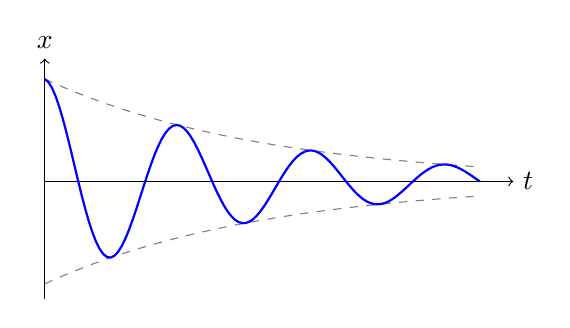
\begin{tikzpicture}[x=.85cm,y=1.3cm]\draw[->](0,0)--(7,0)node[right]{$t$};\draw[->](0,-1.15)--(0,1.2)node[above]{$x$};\draw[dashed,gray,domain=0:6.5,samples=60]plot(\x,{exp(-.3*\x)});\draw[dashed,gray,domain=0:6.5,samples=60]plot(\x,{-exp(-.3*\x)});\draw[blue,thick,domain=0:6.5,samples=120]plot(\x,{exp(-.3*\x)*cos(180*\x)});\end{tikzpicture}
\end{center}
\section{Ví dụ có lời giải}
\subsection*{Ví dụ 3.1}
Với m=0,5 kg, k=8 N/m, x0=0,1 m, v0=-0,2 m/s, không cản, tìm x(t), biên độ.

\textbf{Lời giải.} $\omega_0=4$ rad/s. $x=0{,}1\cos4t-0{,}05\sin4t$ m; biên độ $\sqrt{0{,}01+0{,}0025}=0{,}1118$ m.
\subsection*{Ví dụ 3.2}
Giải x''+4x'+4x=0 với x(0)=1, x'(0)=0.

\textbf{Lời giải.} Nghiệm kép -2. $x=(A+Bt)e^{-2t}$. A=1; $x'(0)=B-2A=0$ cho B=2. Vậy $x=(1+2t)e^{-2t}$.
\section{Nhiệm vụ thực nghiệm}
Dùng SIM-D02 so sánh tỉ số cản 0; 0,3; 1; 1,5 cùng li độ đầu và vận tốc 0. Nhận diện dao động, vượt mức, xác lập; không đồng nhất qua 0 với xác lập.
\section{Ứng dụng hiện đại và chuyển giao}
Cảm biến gia tốc vi cơ có thể mô hình bằng khối thử gắn lò xo có cản, kích thích bởi lực quán tính. Cản đánh đổi rung kéo dài với tốc độ đáp ứng. Cản tốt nhất phụ thuộc băng thông, nhiễu và dung sai quá độ, không có một số tối ưu chung.
\section{Chỉ dẫn đọc nguồn}
SJ §13.2, pp. 52–54; SJ ch. 14; SW ch. 5 catalogue locator.
\section{Luyện tập độc lập}
\begin{enumerate}
\item \textbf{PHY201-B-3.1}. Tìm b tới hạn với m=2 kg, k=18 N/m.
\item \textbf{PHY201-B-3.2}. Giải x''+2x'+5x=0, x(0)=0, x'(0)=4.
\item \textbf{PHY201-B-3.3}. Giải x''+5x'+6x=0, x(0)=1, x'(0)=0.
\item \textbf{PHY201-B-3.4}. Hai đỉnh dương liên tiếp 8 cm và 4 cm cách 2 s. Ước lượng \ensuremath{\gamma} và nêu giả thiết.
\end{enumerate}
\chapter{Đáp ứng cưỡng bức, cộng hưởng và mạch AC}
\section{Mục tiêu năng lực}
Suy biên độ và pha xác lập; phân biệt cộng hưởng li độ và dòng; dùng trở kháng và kiểm tra giả thiết.
\section{Lý thuyết và suy dẫn}
Với $m\ddot x+b\dot x+kx=F_0\cos\omega t$, lấy $x_{\rm ss}=\operatorname{Re}(Xe^{i\omega t})$. Thế cho $(k-m\omega^2+ib\omega)X=F_0$, nên biên độ $|X|=F_0/\sqrt{(k-m\omega^2)^2+b^2\omega^2}$, pha trễ $\delta=\arg(k-m\omega^2+ib\omega)$ trong $[0,\pi]$ với cản và tần số dương. Nghiệm tổng còn quá độ thuần nhất; chỉ khi cản dương quá độ mới suy giảm.

Cực tiểu bình phương mẫu bằng đạo hàm theo $\omega$: $2\omega[2m(m\omega^2-k)+b^2]$. Có đỉnh li độ khác 0 nếu $b^2<2mk$ tại $\omega_r=\sqrt{\omega_0^2-2\gamma^2}$. Nếu không, cực đại trên tần số không âm ở 0. Đúng $\omega_0$ với b dương, li độ trễ lực $\pi/2$. Không cản và đúng cộng hưởng thì công thức xác lập hữu hạn mất hiệu lực; nghiệm riêng tăng theo thời gian.

Theo quy ước $e^{i\omega t}$, trở kháng điện trở $Z_R=R$, cuộn cảm $Z_L=i\omega L$, tụ $Z_C=1/(i\omega C)=-i/(\omega C)$. RLC nối tiếp có $Z=R+i(\omega L-1/(\omega C))$, phasor dòng $I=V/Z$. Với biên độ nguồn cố định và R>0, biên độ dòng cực đại tại $\omega_0=1/\sqrt{LC}$ khi cảm kháng và dung kháng triệt tiêu. Khác cộng hưởng li độ cơ vì dòng tương ứng đạo hàm điện tích. Với biên độ đỉnh, công suất trung bình $P=V_0I_0\cos\phi/2=I_0^2R/2$; với RMS không có hệ số 1/2.

Bộ lọc thông thấp RC lấy đầu ra trên C, hàm truyền $H=1/(1+i\omega RC)$. Môđun $1/\sqrt{1+(\omega RC)^2}$, pha $-\arctan(\omega RC)$, tần số góc cắt $1/(RC)$ tại môđun $1/\sqrt2$. Hàm truyền giả sử nguồn áp lý tưởng, tải không đáng kể. Đây là cầu nối động lực bậc nhất với xử lý tín hiệu.
\begin{center}
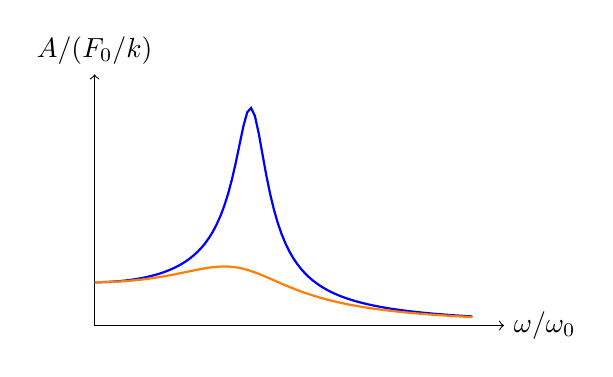
\begin{tikzpicture}[x=2cm,y=.55cm]\draw[->](0,0)--(2.6,0)node[right]{$\omega/\omega_0$};\draw[->](0,0)--(0,5.8)node[above]{$A/(F_0/k)$};\draw[blue,thick,domain=0:2.4,samples=100]plot(\x,{1/sqrt((1-\x*\x)^2+(.2*\x)^2)});\draw[orange,thick,domain=0:2.4,samples=100]plot(\x,{1/sqrt((1-\x*\x)^2+(.8*\x)^2)});\end{tikzpicture}
\end{center}
\section{Ví dụ có lời giải}
\subsection*{Ví dụ 4.1}
Với m=1 kg, k=100 N/m, b=4 kg/s, F0=2 N, tìm biên độ và pha trễ tại \ensuremath{\omega}=10 rad/s; tìm tần số góc cộng hưởng.

\textbf{Lời giải.} Tại 10 rad/s, phần thực mẫu bằng 0, phần ảo 40: $A=2/40=0{,}05$ m; trễ $\pi/2$. $\gamma=2$, $\omega_r=\sqrt{100-8}=\sqrt{92}\approx9{,}592$ rad/s.
\subsection*{Ví dụ 4.2}
RLC nối tiếp R=10 ohm, L=0,1 H, C=100 microfarad, nguồn đỉnh 5 V. Tìm tần số cộng hưởng và công suất trung bình tại đó.

\textbf{Lời giải.} $\omega_0=1/\sqrt{0{,}1(10^{-4})}=316{,}23$ rad/s, $f=50{,}33$ Hz. $I_0=5/10=0{,}5$ A; $P=I_0^2R/2=1{,}25$ W.
\section{Nhiệm vụ thực nghiệm}
Dùng SIM-D03 quét tần số chuẩn hóa tại nhiều tỉ số cản. Tìm đỉnh, đối chiếu dịch chuyển dự đoán, giải thích vì sao đỉnh cao có thể bất lợi cho an toàn kết cấu.
\section{Ứng dụng hiện đại và chuyển giao}
Mạch đầu vào cảm biến RC lý tưởng R=10 kilohm, C=10 nanofarad cho RC=0,0001 s, tần số cắt khoảng 1592 Hz. Ở 10 kHz, độ lợi khoảng 0,157. Lọc giảm nhiễu tần số cao nhưng cũng giảm tín hiệu nhanh hữu ích; chọn băng thông theo mục tiêu đo.
\section{Chỉ dẫn đọc nguồn}
SJ ch. 42, p. 130 (outline only, not full derivation); Swiss ch. 5 and 11 catalogue locators; Chasnov ODE extension.
\section{Luyện tập độc lập}
\begin{enumerate}
\item \textbf{PHY201-B-4.1}. Với \ensuremath{\omega}0=5 rad/s, \ensuremath{\gamma}=1 rad/s, tính tần số góc cộng hưởng li độ.
\item \textbf{PHY201-B-4.2}. Với \ensuremath{\omega}0=4 rad/s, \ensuremath{\gamma}=3 rad/s, có đỉnh li độ ở tần số khác 0 không?
\item \textbf{PHY201-B-4.3}. Tại \ensuremath{\omega}=100 rad/s, R=4 ohm, L=0,05 H, C=0,01 F, nguồn đỉnh 10 V. Tìm trở kháng, biên độ dòng và pha trễ.
\item \textbf{PHY201-B-4.4}. Bộ lọc thông thấp RC có RC=0,02 s. Tìm độ lợi và pha tại \ensuremath{\omega}=50 rad/s, diễn giải.
\end{enumerate}
\chapter*{Tài liệu và mô phỏng}
Tan Chien Hao (2024). \textit{Freshman Physics}.\par
Swiss Physics Olympiad Script, 3rd ed. (2019), catalogue locators pending recheck.\par
\url{https://www.math.ust.hk/~machas/differential-equations.pdf}\par
\url{https://diavn.github.io/truongchuyen/physics-curriculum.html}\par
\url{https://diavn.github.io/truongchuyen/physics-dynamics-lab.html}
\appendix
\chapter{Lời giải đầy đủ}
\section{ODE bậc nhất và quá trình hồi phục}
\begin{enumerate}
\item \textbf{PHY201-B-1.1}. $y=8e^{-3t}$; $e^{-3t}=1/2$ cho $t_{1/2}=\ln2/3$.
\item \textbf{PHY201-B-1.2}. $U=4e^{-1/0{,}5}=4e^{-2}\approx0{,}541$ V.
\item \textbf{PHY201-B-1.3}. $v_T=mg/b=20$ m/s; $\tau=m/b=2$ s; $v(2)=20(1-e^{-1})=12{,}64$ m/s.
\item \textbf{PHY201-B-1.4}. Nhân $e^t$: $(e^ty)'=1$. Tích phân $e^ty=t$, nên $y=te^{-t}$. Đạo hàm $(1-t)e^{-t}$ cộng y bằng $e^{-t}$.
\end{enumerate}
\section{Số phức, dạng Euler và giản đồ pha}
\begin{enumerate}
\item \textbf{PHY201-B-2.1}. $2-6i+i-3i^2=5-5i$.
\item \textbf{PHY201-B-2.2}. $r=\sqrt2$, $\phi=-3\pi/4$, nên $z=\sqrt2e^{-3i\pi/4}$.
\item \textbf{PHY201-B-2.3}. $X=0{,}1e^{0{,}3i}$; $V=i20X=2e^{i(0{,}3+\pi/2)}$; $v=-2\sin(20t+0{,}3)$ m/s.
\item \textbf{PHY201-B-2.4}. $2A|\cos(\delta/2)|=4\cos60^\circ=2$.
\end{enumerate}
\section{ODE bậc hai: dao động tự do và tắt dần}
\begin{enumerate}
\item \textbf{PHY201-B-3.1}. $b_c=2\sqrt{mk}=2\sqrt{36}=12$ kg/s.
\item \textbf{PHY201-B-3.2}. Nghiệm $-1\pm2i$. $x=e^{-t}(A\cos2t+B\sin2t)$; A=0, 2B=4, nên $x=2e^{-t}\sin2t$.
\item \textbf{PHY201-B-3.3}. Nghiệm -2,-3; $A+B=1$, $-2A-3B=0$, cho A=3,B=-2. $x=3e^{-2t}-2e^{-3t}$.
\item \textbf{PHY201-B-3.4}. $\gamma=\ln(8/4)/2=\ln2/2\approx0{,}347$ s$^{-1}$. Giả sử dao động tự do cản nhớt tuyến tính và hai đỉnh cùng dấu.
\end{enumerate}
\section{Đáp ứng cưỡng bức, cộng hưởng và mạch AC}
\begin{enumerate}
\item \textbf{PHY201-B-4.1}. $\omega_r=\sqrt{25-2}=\sqrt{23}\approx4{,}796$ rad/s.
\item \textbf{PHY201-B-4.2}. $\omega_0^2-2\gamma^2=16-18<0$. Không; cực đại tại tần số 0.
\item \textbf{PHY201-B-4.3}. $Z=4+i(5-1)=4+4i$. $|I|=10/(4\sqrt2)=1{,}768$ A; dòng trễ áp $\pi/4$.
\item \textbf{PHY201-B-4.4}. $\omega RC=1$, nên độ lợi $1/\sqrt2$, pha $-\pi/4$. Đây là điểm cắt: biên độ đầu ra 70,7 phần trăm đầu vào.
\end{enumerate}
\end{document}
